
\lhead[\chaptername~\thechapter]{\rightmark}


\rhead[\leftmark]{}


\lfoot[\thepage]{}


\cfoot{}


\rfoot[]{\thepage}


\chapter{A comparison of various architectures}


\section{Overview}

Multicores and Systems on Chip (SoCs) require efficient inter-module
interconnection providing for the required communications at a low
cost. Using the previously defined costs , using area and power we
would try to analyze how the different architectures fare : a shared
bus, a segmented bus and a point-to-point interconnect. For each architecture
we discuss analytical expressions for area, power dissipation and
operating frequency as well as asymptotic limits of these functions. 

We show how NoCs actually provide scalability advantages over other
architecture and thus are better prospects for the future. While the
costs associated with a chip is measured in terms of power and area
, the most commonly accepted measure of performance is QoS. QoS is
usually associated with throughput and latency. 


\section{NoC topology}

We assume a very basic mesh network topology for the NoCs discussed.


\subsection{NoC communication fabric}

Packets carry routing information, command and payload. While the
payload delivers the real data , some overhead is unavoidable , akin
to the large scale networks. The command field identifies the payload,
specifying the type of operation. The packet is divided into multiple
flits following . Flit transfer over the inter-router link may be
controlled by handshake. 


\subsection{NoC routers}

NoC comprises routers interconnected by point-to-point links. Network
topology can vary depending on system needs and module sizes and placement.
Each system module is connected to a router (Fig. 1) via a standard
interface, whose bandwidth might be adapted to the communication needs
of that module. The bandwidth of each inter-router link is similarly
adjusted to accommodate the expected traffic and fulfill QoS requirements
at the specific link. The link bandwidth can be controlled by the
link frequency and link width.

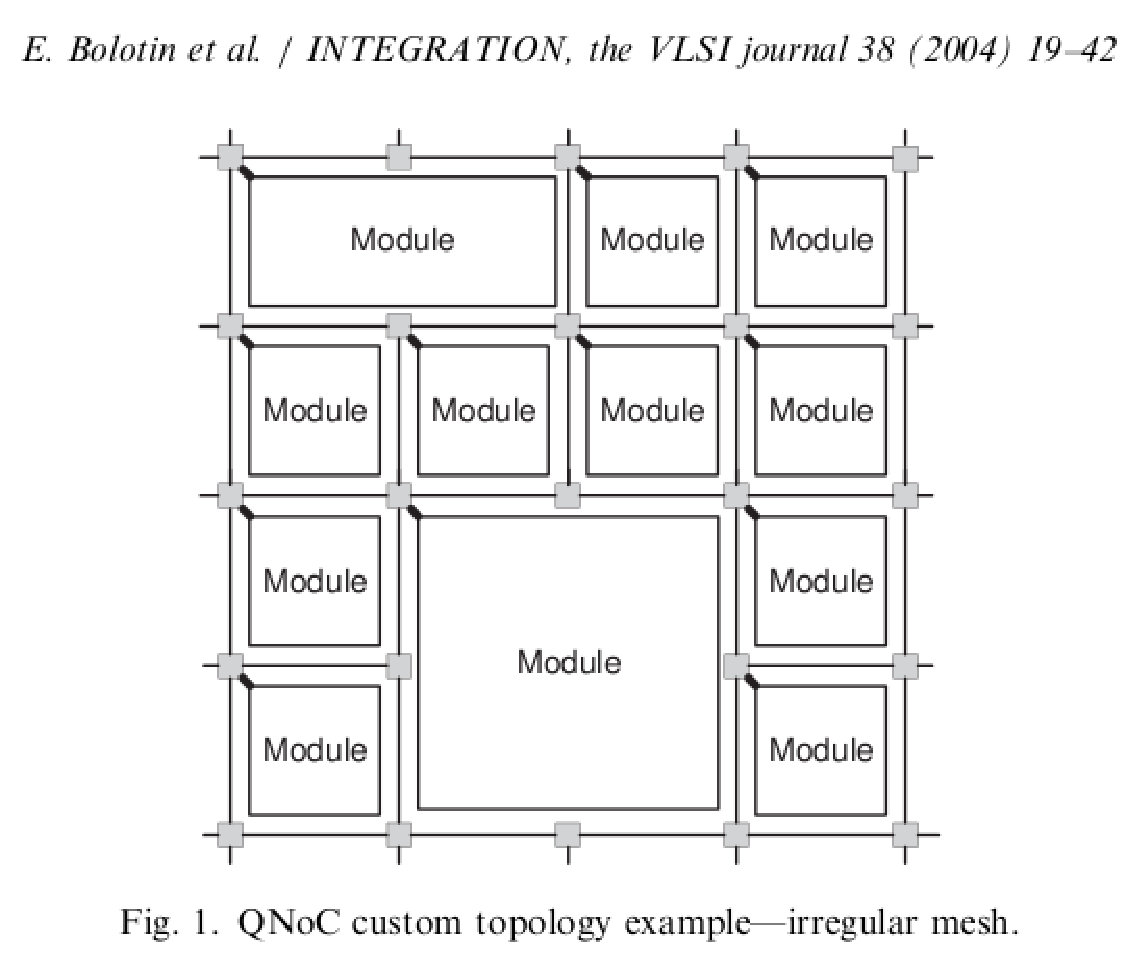
\includegraphics[width=7cm]{images/1}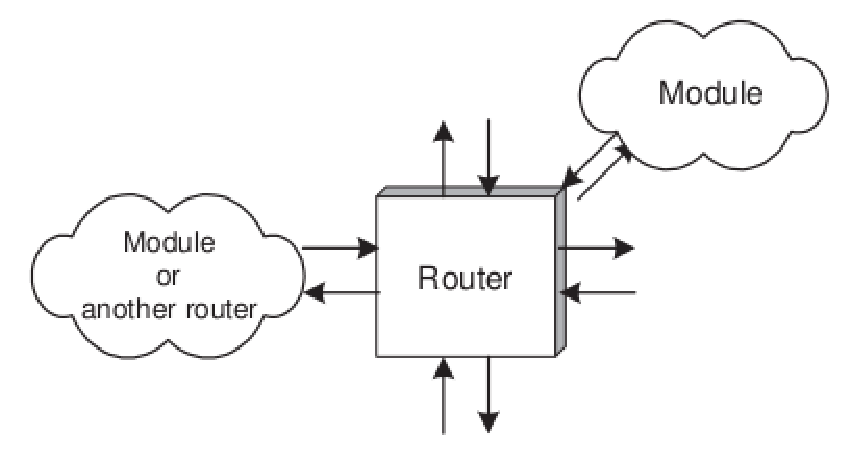
\includegraphics[scale=0.4]{images/2}


\subsection{NoC IPs}

The IPs consist of the functional part of NoC that is directly involved
in computations. It may be a memory module , a generic processor or
a special purpose processor. The variety of IP cores is as wide as
that of in SoCs.


\section{Cost Comparisons}


\subsection{Various Topolgies}


\subsubsection{NoC}

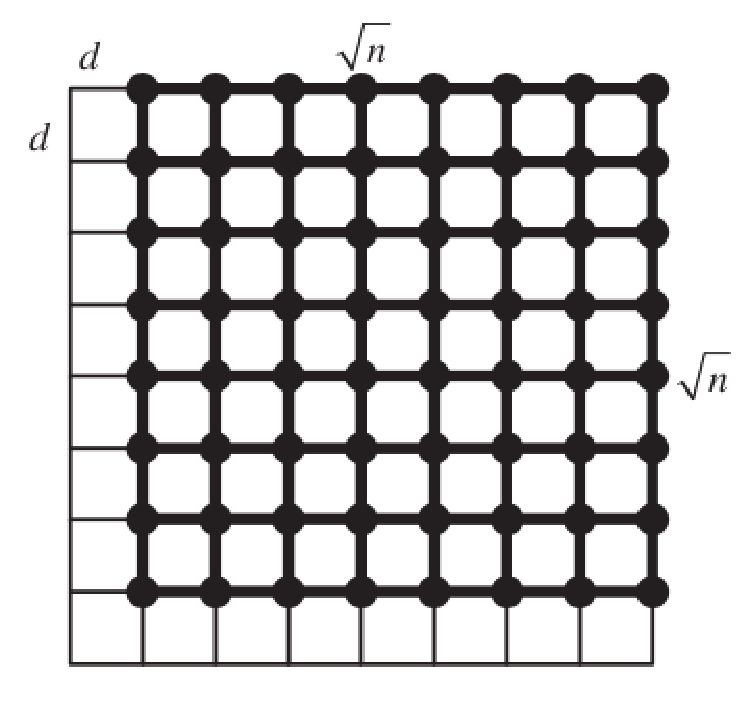
\includegraphics[width=7cm]{images/3}\cite{Bolotin:2004:CCN:1056481.1056484}%
\framebox{\begin{minipage}[t]{0.1\columnwidth}%
Fig. 2%
\end{minipage}}

Consider n system modules interconnected by a NoC (Fig. 2). Each module
is connected to a router using a standard interface, and the routers
are interconnected in a mesh topology. For the NoC case, we assume
that the silicon cost of minimal buffer routers and simple module
interfaces are comparable to similar costs of other solutions (such
as bus multiplexers, bus interfaces, etc.). Moreover, these costs
are linear with the number of modules and therefore do not change
the asymptotic comparison. 


\subsubsection{Unsegmented Bus}

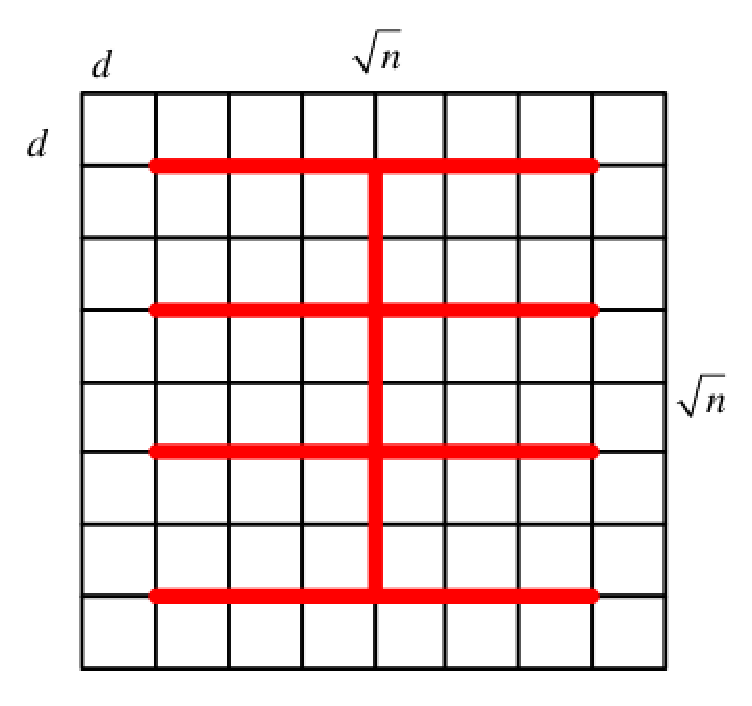
\includegraphics[width=7cm]{images/4}\cite{Bolotin:2004:CCN:1056481.1056484}%
\framebox{\begin{minipage}[t]{0.1\columnwidth}%
Fig. 3%
\end{minipage}}

The NS-Bus is a simple shared bus, connecting all modules in the system
and laid out as a minimal spanning tree (Fig. 3). It consists of a
single segment and has no parallelism (only one transaction is active
at a time). 


\subsubsection{Segmented Bus}

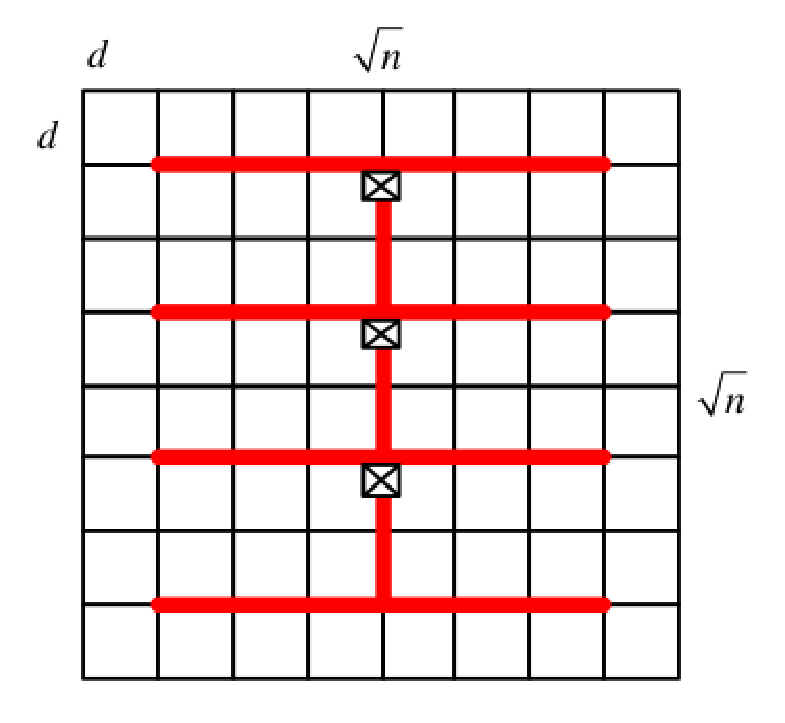
\includegraphics[width=7cm]{images/5}\cite{Bolotin:2004:CCN:1056481.1056484}%
\framebox{\begin{minipage}[t]{0.1\columnwidth}%
Fig. 4%
\end{minipage}}

The S-Bus is the most widely used SoC interconnection architecture,
primarily because a long shared bus that interconnects all system
modules is not feasible in systems consisting of many communicating
nodes. We assume a similar topology as NS-Bus, but segmented into
n/2 identical sections (of the same length, width and frequency).
The interconnection is established by bridges, as in Fig. 4. The S-Bus
has more parallelism, because the segments are independent. Also,
the capacitance of each segment is substantially reduced relative
to that of the NS-Bus, allowing the S-Bus to operate at higher frequencies.
This structure was a deviation from the primitive single bus architectures
, and a move towards the connection based ones.


\subsubsection{Point to Point}

Consider n modules arranged in a mesh and interconnected point-to-point
with links that are routed in an X-Y fashion, similar to the NoC.
Note that here , the wires are routed instead of packets. This has
the direct implication that the net wire length explodes with the
network size. We are forced to resort to such an architecture because
the 2D chips enforce a constraint of planarity of topology (ie the
wires cannot intersect). The view of network is exactly same as that
of Fig 2.


\subsection{Asymptotic Bounds}

Following the aforementioned specifications \cite{Bolotin:2004:CCN:1056481.1056484}
arrived at the following asymptotic complexities.

\begin{tabular}{|c|c|c|c|}
\hline 
Architecture & Total Area & Power dissipation & Operating frequency\tabularnewline
\hline 
\hline 
NS - Bus & O($n^{3}\sqrt{n}$) & O($n\sqrt{n}$) & O($\tfrac{1}{n^{2}}$)\tabularnewline
\hline 
S - Bus & O($n^{2}\sqrt{n}$) & O($n\sqrt{n}$) & O($\tfrac{1}{n}$)\tabularnewline
\hline 
NoC & O($n$) & O($n$) & O(1)\tabularnewline
\hline 
PTP & O($n^{2}\sqrt{n}$) & O($n\sqrt{n}$) & O($\tfrac{1}{n}$)\tabularnewline
\hline 
\end{tabular}

\ \\

The total area: 
\begin{itemize}
\item Since the NS-bus operates at a very slow frequency (decreasing as
O($\tfrac{1}{n^{2}}$) ) and has no parallelism, it has to be made
excessively wide to provide the same effective in order bandwidth
as the NoC.As a result, its width grows as O($n^{2}\sqrt{n}$) and
its length grows as O($n$), so that its total area cost function
grows as O($n^{3}\sqrt{n}$)
\item The S-Bus is O($n$) faster than the NS-Bus because each segment is
O($n$) shorter and it employs O($n$) segments in parallel, but since
the average number of hops traversed on the segmented bus is also
O($n$) ; it results in no parallelism. Thus, the S-bus requires O($n$)
fewer links than the NS-bus and its total area cost function is O($n^{2}\sqrt{n}$)
\item The NoC wire-cost increases only as O($n$)
\item In PTP the average link frequency O($n$) slower than in the NoC (longer
links with higher capacitance).
\item The, link length grows as O($n^{2}\sqrt{n}$) and since the link width
is asymptotically O(1), its total area also grows as O($n^{2}\sqrt{n}$)
\end{itemize}
\ \\

The power dissipation cost function:
\begin{itemize}
\item Power dissipated by all architectures is proportional to the product
of operating frequency and total wire length. 
\end{itemize}
\ \\

Thus , our analysis clearly shows an asymptotic supremacy of the NoC.
Our assumptions being, a uniform traffic distribution and assuming
that load capacitance depends only on the interconnect (ignoring the
capacitance of system module ports). It is notable that the above
assumptions only put NoC on the lower ground. Non uniform traffic
, mostly local, favours NoC , as does the inclusion of port capacitance.
As the technology improves, NoC is the only communication architecture
where the links become shorter and less vulnerable to delays and noise. 




